\section{Introduction}

In genomic analysis, to assess whether
there is a significant association between two sets of genomic ranges, 
one must choose an appropriate null model \citep{reviewdilemma2014,kanduri2018}.
\rev{Here we use the term ``ranges'' to denote a set of genomic features defined by sequence name (e.g. chromosome), starting basepair, ending basepair, and optionally strand and other metadata variables}.
For example, an enrichment of ATAC-seq peaks near certain genes
may indicate a regulatory relationship \citep{lee2020fluent}, 
and enrichment of GWAS SNPs near tissue-specific ATAC-seq peaks may
suggest mechanisms underlying the GWAS trait.
Such analyses rely on specifying a null distribution, where one
strategy is to uniformly shuffle one set of the
genomic ranges in the genome, possibly considering a set of
excluded regions \rev{where ranges should not be placed} \citep{excluderanges}.
However, uniformly distributed null sets will not exhibit the
clumping property common with genomic regions.
Using an overly simplistic null distribution that doesn't take into
account local dependencies could result in misleading conclusions.
More sophisticated methods exist, for example
GAT, which allows for controlling by local GC content
\citep{GAT_2013}, and regioneR, which implements a circular shift to
preserve the clumping property \citep{gel2016regioner}.
The block bootstrap \citep{politis1999subsampling}
provides an alternative, where one instead generates
random sets of ranges by sampling large blocks of ranges from the
original set with replacement, as originally proposed for 
genomic data by \citet{bickel2010subsampling} in Genome Structure
Correlation (GSC).
Using the block bootstrap is more
computationally intensive than simple shuffling, and so GSC implements
a strategy of swapping pairs of blocks to compute overlaps, while
avoiding a genome-scale bootstrap.

Here we describe the \bootranges software, with efficient
vectorized code for performing block bootstrap sampling of genomic ranges
\rev{stored as \granges objects in R/Bioconductor}
\citep{lawrence2013software}.
\rev{\bootranges is part of a modular analysis workflow, where bootstrapped
ranges can be analyzed at block or genome scale using tidy
analysis with packages including \plyranges \citep{lee2019plyranges},
and \tidybulk \citep{mangiola2021tidybulk}.}
%%\rev{and \tidybulk \citep{mangiola2021tidybulk}}.
We provide recommendations for genome segmentation and block length
motivated by analysis of example datasets.
We demonstrate how \bootranges can be incorporated into complex
downstream analyses, including choosing the thresholds during
enrichment analysis and single-cell multi-omics.
\rev{\bootranges is distributed as part of the \nullranges R/Bioconductor package.
If directly controlling for nuisance covariates when building
background sets is of interest, the sister function \matchranges \citep{Davis2022matchranges}
may be more appropriate, see the package documentation for an overview of
\bootranges and \matchranges.}

\section{Features}

\bootranges offers a ``segmented'' block bootstrap:
since the distribution of ranges in the genome exhibits multi-scale
structure, we follow the logic of \citet{bickel2010subsampling} and consider to
perform block bootstrapping within \textit{segments} of the genome, which are
more homogeneous in their range density.
\rev{A simple ``unsegmented'' block bootstrap is additionally
  implemented but the segmented version is generally recommended.  We
  consider various genome segmentation procedures, segmenting on gene
  density, or pre-existing annotations}, e.g. Giemsa bands or
published segmentations.
The genome segments define large (e.g. on the order of ${\sim}1$ Mb),
relatively homogeneous segments from which to sample blocks
(\cref{fig:framework}A).
\rev{Blocks are sampled across segments that are in the same
  segmentation \textit{state} (see Supplementary for details).} 
The input for the workflow is region sets \bm{$x$} and
\bm{$y$}, with optional metadata columns that can be
used for computing a more complex test statistic than overlaps.
Given a segmentation and block length $L_b$, a \textit{BootRanges}
object is generated, which concatenates ranges across bootstrap
iterations. This \textit{BootRanges} object can be manipulated with \plyranges
to derive the bootstrap distribution of test statistics $\{s_r\}$ and a
bootstrap p-value:
$ \frac{1}{R} \sum_{r=1}^R \mathbb{I}_{\{s_r > s_\text{obs}\}} $ (\cref{fig:framework}B).
The \bootranges algorithms are explained schematically in Supplementary \cref{sec:algorithm}.


\begin{figure}[t]
\centering
\setlength{\abovecaptionskip}{-0.05cm}
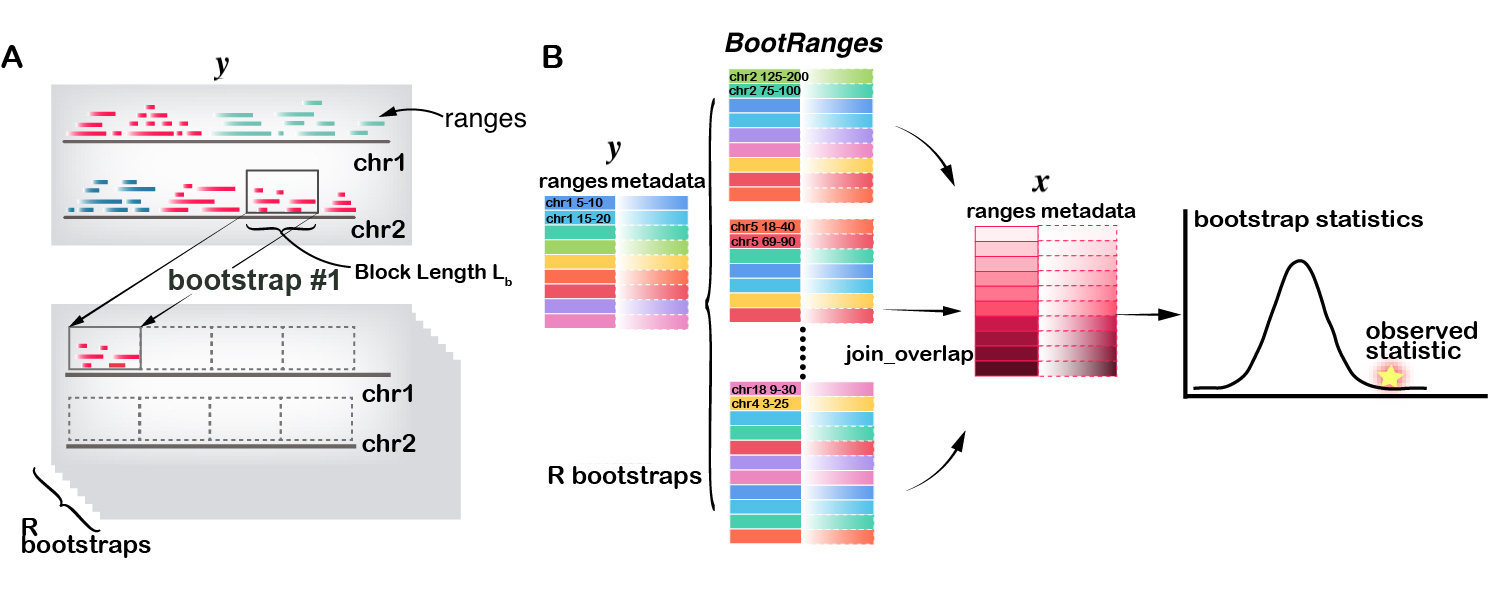
\includegraphics[scale=0.16]{Figures/bootRanges.jpeg}
\caption{
  \rev{Schematic overview of the segmented block bootstrap 
  for assessing significance of an observed statistic.
  A) In each bootstrap sample, 
  new sets of ranges are created by resampling blocks of length 
  $L_b$, with replacement, from the original set \bm{$y$}. 
  Color represents genome segmentation states, such that blocks 
  may be sampled across chromosomes, from within the same 
  segmentation state.
  B) Workflow for testing association between 
  ranges in \bm{$x$} and \bm{$y$},  
  e.g. counting the number of overlapping ranges. 
  First, $R$ bootstrap samples of \bm{$y$} are 
  generated and stored as a \textit{BootRanges} object.
  Then, the bootstrap distribution of test statistics 
  (e.g. count of overlaps) 
  between \bm{$x$} and \textit{BootRanges} is computed.
  Finally, the observed overlap statistic between \bm{$x$} and \bm{$y$} 
  is compared to the bootstrap distribution.}}
\label{fig:framework}
\end{figure}


\section{Application}
\subsection{Test for association between SNPs and peaks}

We first applied \bootranges to determine the significance of the
overlap of liver ATAC-seq
\citep{CURRIN20211169} with SNPs associated with total cholesterol,
bootstrapping the SNPs to assess significance.
%% \mike{Why do we say this? Maybe drop this sentence? 
%% ``As reported by \citet{bickel2010subsampling}, the effect
%% of segmentation did not greatly alter conclusions.''}
\rev{While the observed overlap was significant across many combinations of
various segmentation methods and $L_b$ according to typical p-value cutoff,
the variance of the bootstrap statistics distribution 
and the resulting $z$ score varied across 
segmentation choice, though varying more across block length 
(\cref{fig:result}A-B). The effect of segmentation may be stronger 
in other contexts.}
We used the $z$ score to measure the distance between the observed
statistics and bootstrap distribution in terms of standard deviations.
Overlap rate was defined as the proportion of
SNPs that had peaks within 10kb.
That the variance of the distribution in \cref{fig:result}A for the
unsegmented bootstrap increased with $L_b$ indicated that
ranges are inhomogeneous and
bootstrapping with respect to a genome
segmentation may be a more appropriate choice
\citep{bickel2010subsampling}. 
The decreasing trend using pre-defined segmentation from
Roadmap Epigenomics indicated too many short segments,
where $L_b$ is too close to $L_s$ for effective block randomization.
\rev{To chose an optimal segmentation, 
we noted those for which the variance of the bootstrap distribution 
becomes stable as $L_b$ increases (\cref{fig:result}A).
To choose an optimal $L_b$ range, two aspects were considered:
1) we sought a minimum value of a scaled version of the change 
in the variance of bootstrap statistics distribution across $L_b$, 
as recommended previously \citep{bickel2010subsampling},
and 2) we assessed whether the distribution of inter-range distances  
was preserved, when comparing to the original ranges 
(Supplementary \cref{sec:length}).}
Here $L_s \approx 2$ Mb and $L_b \in [300\textrm{kb},600\textrm{kb}]$ was 
shown to be a good range for segment and block
lengths (\cref{fig:suppfig0}A-C, and Supplementary \cref{sec:liveratac}).
The scientific conclusion of this example was that liver ATAC-seq
peaks were
much closer to total cholesterol SNPs than expected even when placing
blocks of SNPs to match a genome segmentation. 
Shuffling of genomic ranges (Supplementary \cref{sec:shuffle})
resulted in a much higher $z = 18.5$, compared to $z \approx 4$ 
consistent with previous conclusions that shuffling may 
overestimate significance leading to misinterpretation of enrichment.


%\vspace{-0.5cm}
% \newpage
\begin{figure}[H]
\centering% default with `floatrow`
\setlength{\abovecaptionskip}{-0.1cm}
\setlength{\belowcaptionskip}{-0.1cm}
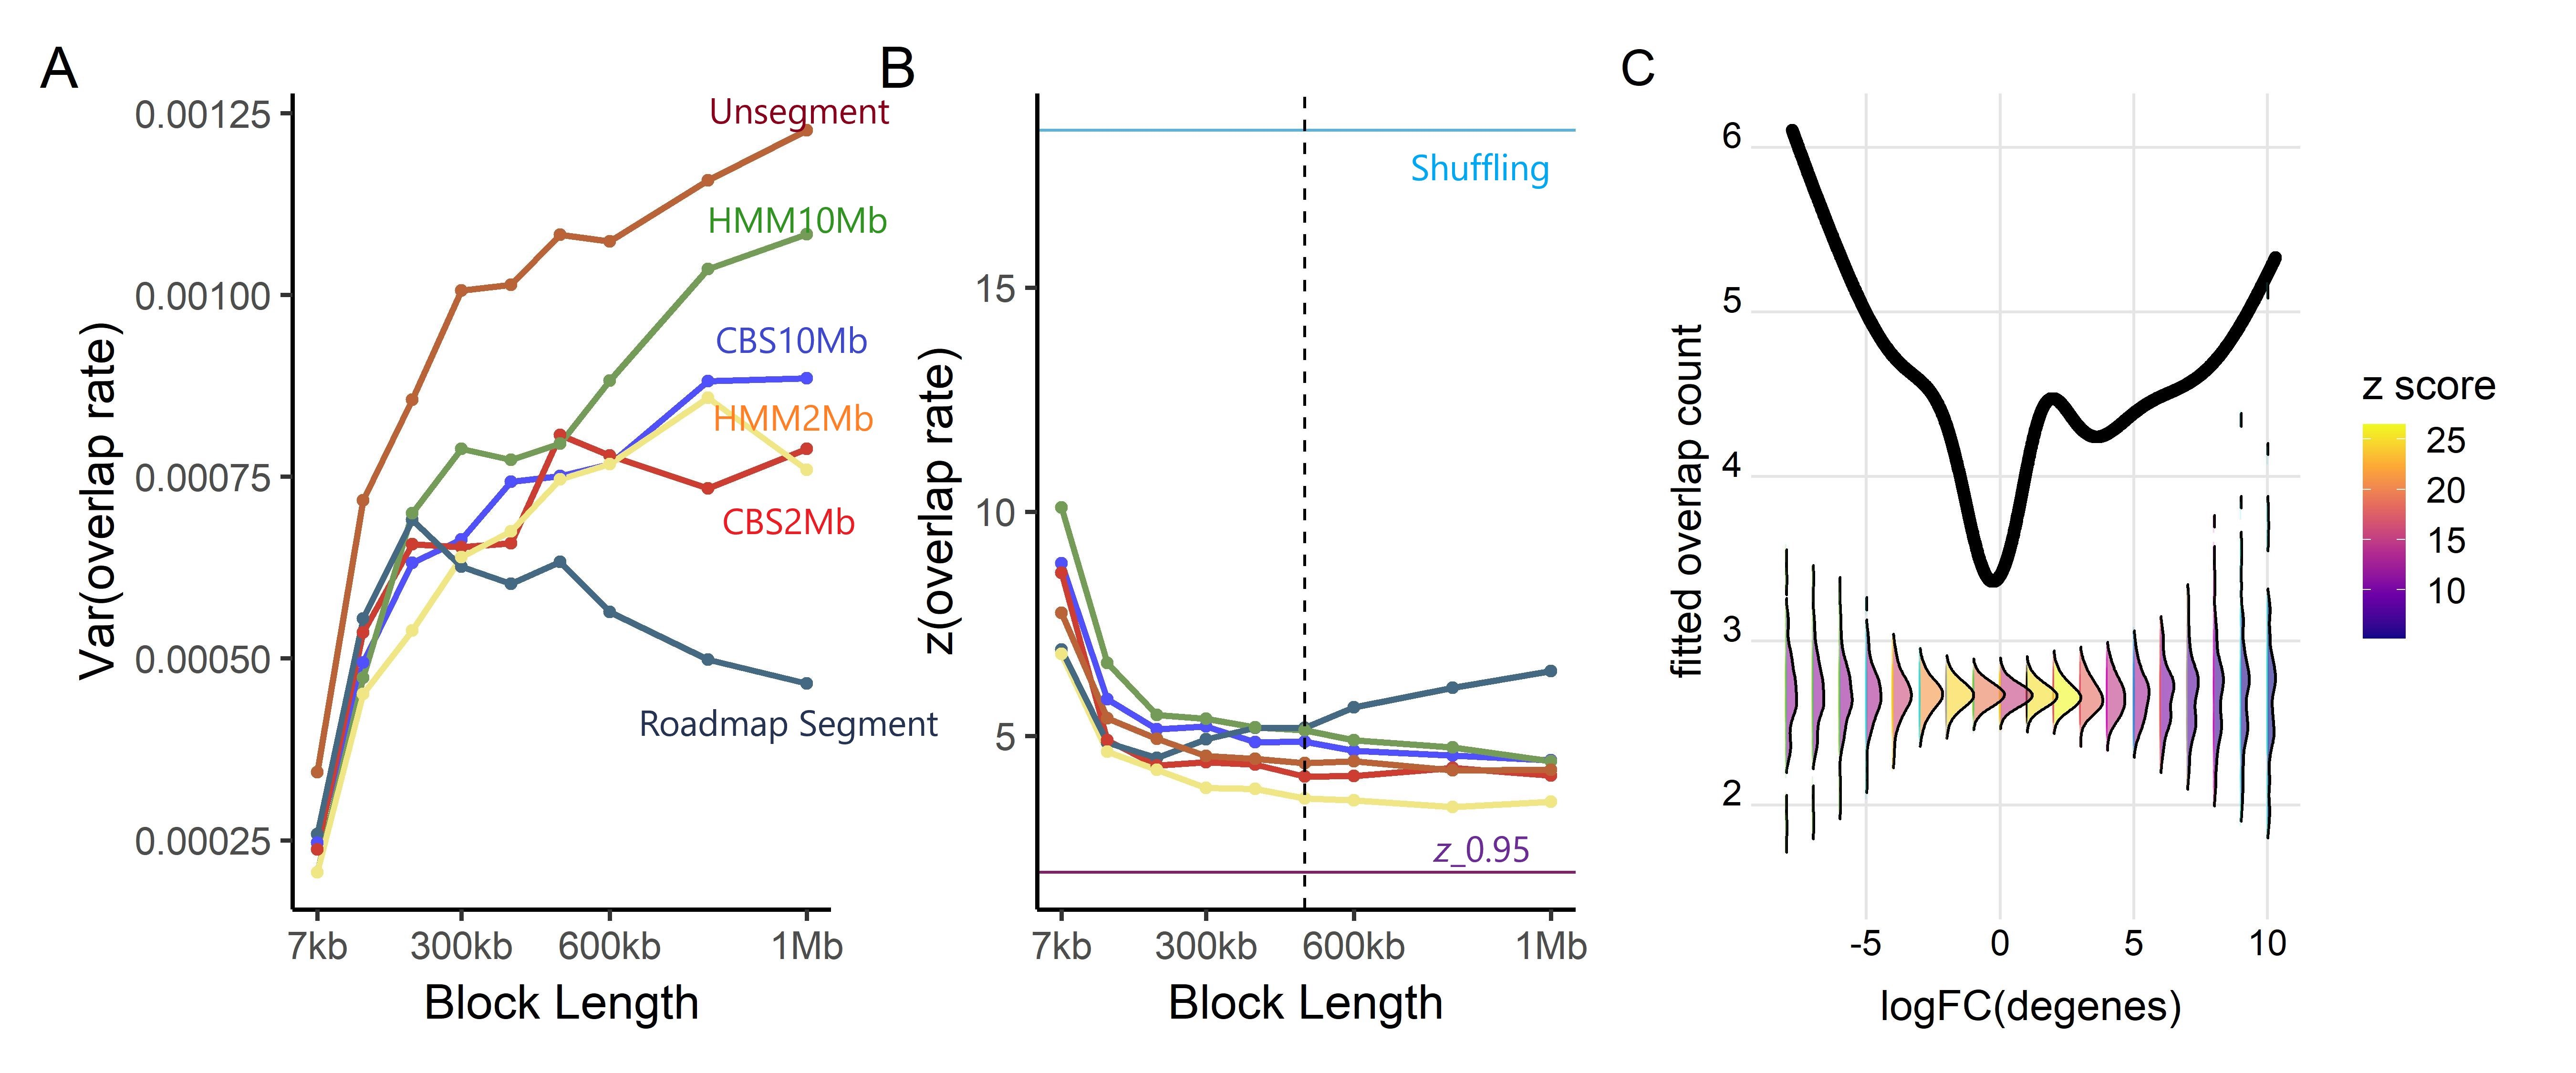
\includegraphics[scale=0.06]{Figures/fig2_3.jpeg}
\caption{
  Parameter selection and overlap analysis.
  A) Variance of the rate of overlaps and,
  B) $z$ score for the overlap,
  for different segmentations and $L_b$ on the liver 
  dataset.
  C) GAM predicted curves for observed (black line) and
  bootstrapped data (densities),
  for the overlap count over gene logFC.
  Conditional densities are colored by the $z$ score for the overlap.
}
\label{fig:result}
%\vspace{-.5cm}
\end{figure}

%% z score, independent of number of bootstraps, was used to measure the
%% distance between the expected value and the observed one according to
%% the standard deviations.
%% the $z = 4.10$ if look at circular binary search(CBS)
%% \citep{cbs} segmentation method with $L_s = 2e6$ and
%% $L_b=5e5$(\cref{fig:result}B).
%% As seen in applications of \citet{bickel2010subsampling}, the effect
%% of segmentation did not greatly alter conclusions, e.g. rejection of
%% the null hypothesis, in this case, although the z score varies greatly
%% among the different segmentations and block lengths.

\subsection{Choosing thresholds for enrichment analysis}
We demonstrated using \bootranges to motivate the choice of data-driven thresholds 
during enrichment analyses. We tested this on a dataset of differential chromatin accessibility and gene expression 
\citep{alasoo2018shared,lee2020fluent} and previous liver ATAC-seq.
A generalized linear model (GLM) with penalized splines was
fit to the overlap count over gene logFC, both for the original
data and to each of the generated null sets.
Conditional densities of splines fit to null sets
were computed at various thresholds to reveal how
the threshold choice would affect the
variance of the bootstrap density and the resulting $z$ score
(\cref{fig:result}C). 
\rev{The observed enrichment with respect to bootstrapped ranges 
varies over the logFC threshold. Instead of picking an arbitrary logFC cutoff, 
these analyses suggested that SNPs with -log10 (\textit{p}-value) $> 8$ and 
genes with $|\textrm{logFC}| > 2$ were sets where the $z$ score reflected 
strong separation of the observed statistic from the bootstrap statistic 
distribution
(\cref{fig:suppfig2}).}


%We demonstrate using \bootranges to motivate the choice of thresholds 
%that are applied to genomic regions during enrichment analyses.
%We tested this on the aforementioned liver ATAC-seq example, and on a
%dataset of differential chromatin accessibility and gene expression 
%\citep{alasoo2018shared,lee2020fluent}.
%A generalized linear model (GLM) with penalized regression splines was
%fit to the overlap rate or count over the $-\log_{10}(p)$ or
%gene logFC, both for the original
%data and to each of the bootstrap datasets.
%Condition densities of splines fit to bootstrap data
%were computed at various thresholds to reveal how
%the threshold choice would affect the
%variance of the bootstrap density and the resulting $z$ score
%(\cref{fig:result}C-D).
%These analyses suggested that $-\log_{10}(p) = 8$ and
%$|\textrm{logFC}| = 2$
%are optimized thresholds where the $z$ score was highest
%(\cref{fig:suppfig2}A-B).

%We found that the $z$ score was highest when $-\log_{10}(p) = 8$
%(\cref{fig:suppfig2}A),
%and when $\textrm{|logFC|} = 2$(\cref{fig:suppfig2}B).
%(\cref{fig:suppfig2}B).
%% from \textit{gam} function in the
%% \emph{mgcv} R package were fitted and \textit{predict\_gam} function
%% in the \emph{tidymv} R package were predicted on observed and each
%% null sets.
%% $$
%% \setlength{\abovedisplayskip}{3pt}
%% \setlength{\belowdisplayskip}{3pt}
%% log \left( \frac{\pi}{1-\pi} \right) = \beta_0  + f (-log_{10}p), log(\mu) = \beta_0 + f (log_{FC})
%% $$ 
%% for rate and count-based statistic, separately.
%% All generated 95\%
%% percentile intervals at the same time across a range of effect sizes
%% were displayed by conditional density plot 

\subsection{Identification of gene-promoter pairs by single-cell multi-omics}
We applied \bootranges to
%Chromium Single Cell Multiome
single cell multiome
ATAC-seq and RNA-seq, to assess the correlation ($\rho$) of log counts for the two
modalities for all pairs of genes and peaks, across
14 cell types (pseudo-bulk). Across all genes, we observed
$\bar{\rho} = 0.33$, which was 
significantly higher than the bootstrap correlation mean
(\cref{fig:suppfig3}A, $\bar{\rho}_{R} = 0.007$). As expected, RNA
and ATAC measured at local peaks had similar cell-type-specificity.
Additionally, the average gene-peaks correlation per gene can be
computed and compared to a bootstrap distribution to
identify gene-promoter pairs that were significantly correlated across
cell types (\cref{fig:suppfig3}B-C).

\subsection{Simulation}

\rev{To assess the accuracy of the bootstrap distribution in capturing
the true null distribution, we generated a simulation in which
there was no true association between $\bm{x}$ and $\bm{y}$. 
We compared the bootstrap distribution using \bootranges 
with that using shuffling. Details are provided in Supplementary
\cref{sec:sim}. 
Given that there is no true association, we would expect false
positive rate (FPR) $\approx \alpha$, 
the threshold for significance, if the randomization method was 
successfully approximating the data generating distribution for $\bm{y}$.
We found that \bootranges could achieve an FPR near $\alpha$. 
Shuffling however generated a distribution of statistics
with similar mean as the original distribution, but with much lower
variance.
Therefore the FPR for shuffling in this simulation was relatively high 
and would lead to overestimation of the significance of the overlap 
(\cref{fig:simulation}).}

To compare speed, we ran \bootranges and GSC on
ENCODE kidney and bladder ChIP-seq. The average time to
block bootstrap the genome using \bootranges was 0.30s and
0.37s with overlap computation. A comparable analysis with GSC took
7.56s.

%\vspace*{-20pt}
\section{Conclusion}

\bootranges efficiently generates null models of genomic ranges preserving 
local genomic correlations, and can be used easily in combination with
other range-based tools such as \plyranges.
It has great flexibility in various disciplines (e.g. identify
putative transcription factor binding site according to enriched peak
regions).

\bootranges is distributed in the \nullranges Bioconductor package,
while all of the R scripts and data used in this paper are available
at the following GitHub repository: 
\url{https://github.com/Wancen/bootRangespaper}.

%\vspace*{-20pt}

\section*{Funding}
CZI EOSS and R01-HG009937 to M.I.L, NIH R35-GM128645 to D.H.P.

%\vspace*{-20pt}
